% !TEX root = main.tex

\section{Optimal control of Pitch/Travel without Feedback}
\subsection{Continuous time state space model}
The continuous time system can be written as $\mathbf{\dot{x}} = \mathbf{A}_c\mathbf{x}+ \mathbf{B}_c{u}$, with
\begin{subequations}
    \begin{align}
        \mathbf{x} &= \begin{bmatrix}
            \lambda\\
            r\\
            p\\
            \dot{p}
        \end{bmatrix}\\
        \mathbf{A}_c &= \begin{bmatrix}
            0 & 1 & 0 & 0\\
            0 & 0 & -K_2 & 0\\
            0 & 0 & 0 & 1\\
            0 & 0& -K_1K_{pp} & -K_1K_{pd}
        \end{bmatrix} \\
        \mathbf{B}_c &= \begin{bmatrix}
            0\\
            0\\
            0\\
            K_1K_{pp}
        \end{bmatrix}
    \end{align}
\end{subequations}

This is the model given in the exercise text. It models the helicopter together with a pitch controller. The model inputs are set points for the pitch controller.

\subsection{Discretization}
The system was discretized using forward Euler:
\begin{equation}
    \mathbf{\dot{x}} = \mathbf{A}_c\mathbf{x}_k + \mathbf{B}_c{u}_k \approx \frac{\mathbf{x}_{k+1}-\mathbf{x}}{h}
\end{equation}

Rearranging, we get
\begin{equation}
    \mathbf{x}_{k+1} = (\mathbf{A}_ch + \mathbf{I})\mathbf{x}_k + h\mathbf{B}_c{u}_k
\end{equation}

and we see that
\begin{subequations}
    \begin{align}
        \mathbf{A}_d &= \mathbf{A}_ch+\mathbf{I} \\
        \mathbf{B}_d &= h\mathbf{B}_c
    \end{align}
    \label{eq:eulerfwd}
\end{subequations}

\begin{subequations}
    \begin{align}
        \mathbf{A_d} &= \begin{bmatrix}
        1 & h & 0 & 0\\
        0 & 1 & -hK_2 & 0\\
        0 & 0 & 1 & h\\
        0 & 0 & -hK_1K_{pp} & 1-hK_1K_{pd}
        \end{bmatrix}\\
        \mathbf{B_d} &= \begin{bmatrix}
        0\\
        0\\
        0\\
        hK_1K_{pp}
    \end{bmatrix}
    \end{align}
\end{subequations}

It should be noted that forward Euler has rather awful precision and stability properties compared to other discretization methods. On the plus side, it is intuitive and easy to implement.

\subsection{Optimal trajectory planning}
\begin{lstlisting}
    [z,lambda] = quadprog(Q,c,[],[], Aeq, beq, vlb, vub);
\end{lstlisting}

The optimal trajectory \todo{what optimal trajectory?} was calculated using \texttt{quadprog}, which takes a weight matrix \texttt{Q}, vector \texttt{c} (from the cost function $x^TQx + c^Tx$), inequality constraints matrices \texttt{A}, \texttt{B}, equality constraints \texttt{Aeq}, \texttt{Beq} and lower and upper bounds \texttt{vlb}, \texttt{vub} on the inputs, and returns a vector z with the optimal trajectory for all the states, along with a vector $\lambda$ containing the Lagrange multipliers at the solution.

\begin{lstlisting}
    Q1(1,1) = 1;
    ...
    P1 = 10;
    Q = 2*genq2(Q1,P1,N,M,mu);
    c = zeros(N*mx+M*mu,1);
    ...
    Aeq = gena2(A1,B1,N,mx,mu);
    beq = zeros(size(Aeq,1),1);
    ...
    [vlb,vub] = genbegr2(N,M,xl,xu,ul,uu);
\end{lstlisting}
The weight matrix \texttt{Q} was generated using the function \texttt{genq2}, and \texttt{c} is a vector of zeros. \texttt{Aeq} was generated using the function \texttt{gena2}, while \texttt{beq} is a vector of zeros. The constraints on the inputs were implemented using the given function \textt{genbegr2}.

Finally, \texttt{mx} denotes the number of states, \texttt{mu} the number of inputs, \texttt{N} the time horizon for states and \texttt{M} the time horizon for inputs. For a more detailed description of the above functions, see Appendix \cref{appendix:A}.

The optimal input and optimal trajectory for the travel rate $\lambda$ are shown in \cref{fig:optimal_inputs} and \cref{fig:optimal_lambda}, respectively.
%\clearpage %Let LaTeX handle this

\begin{figure}[h]
    \centering
    \makebox[\textwidth][c]{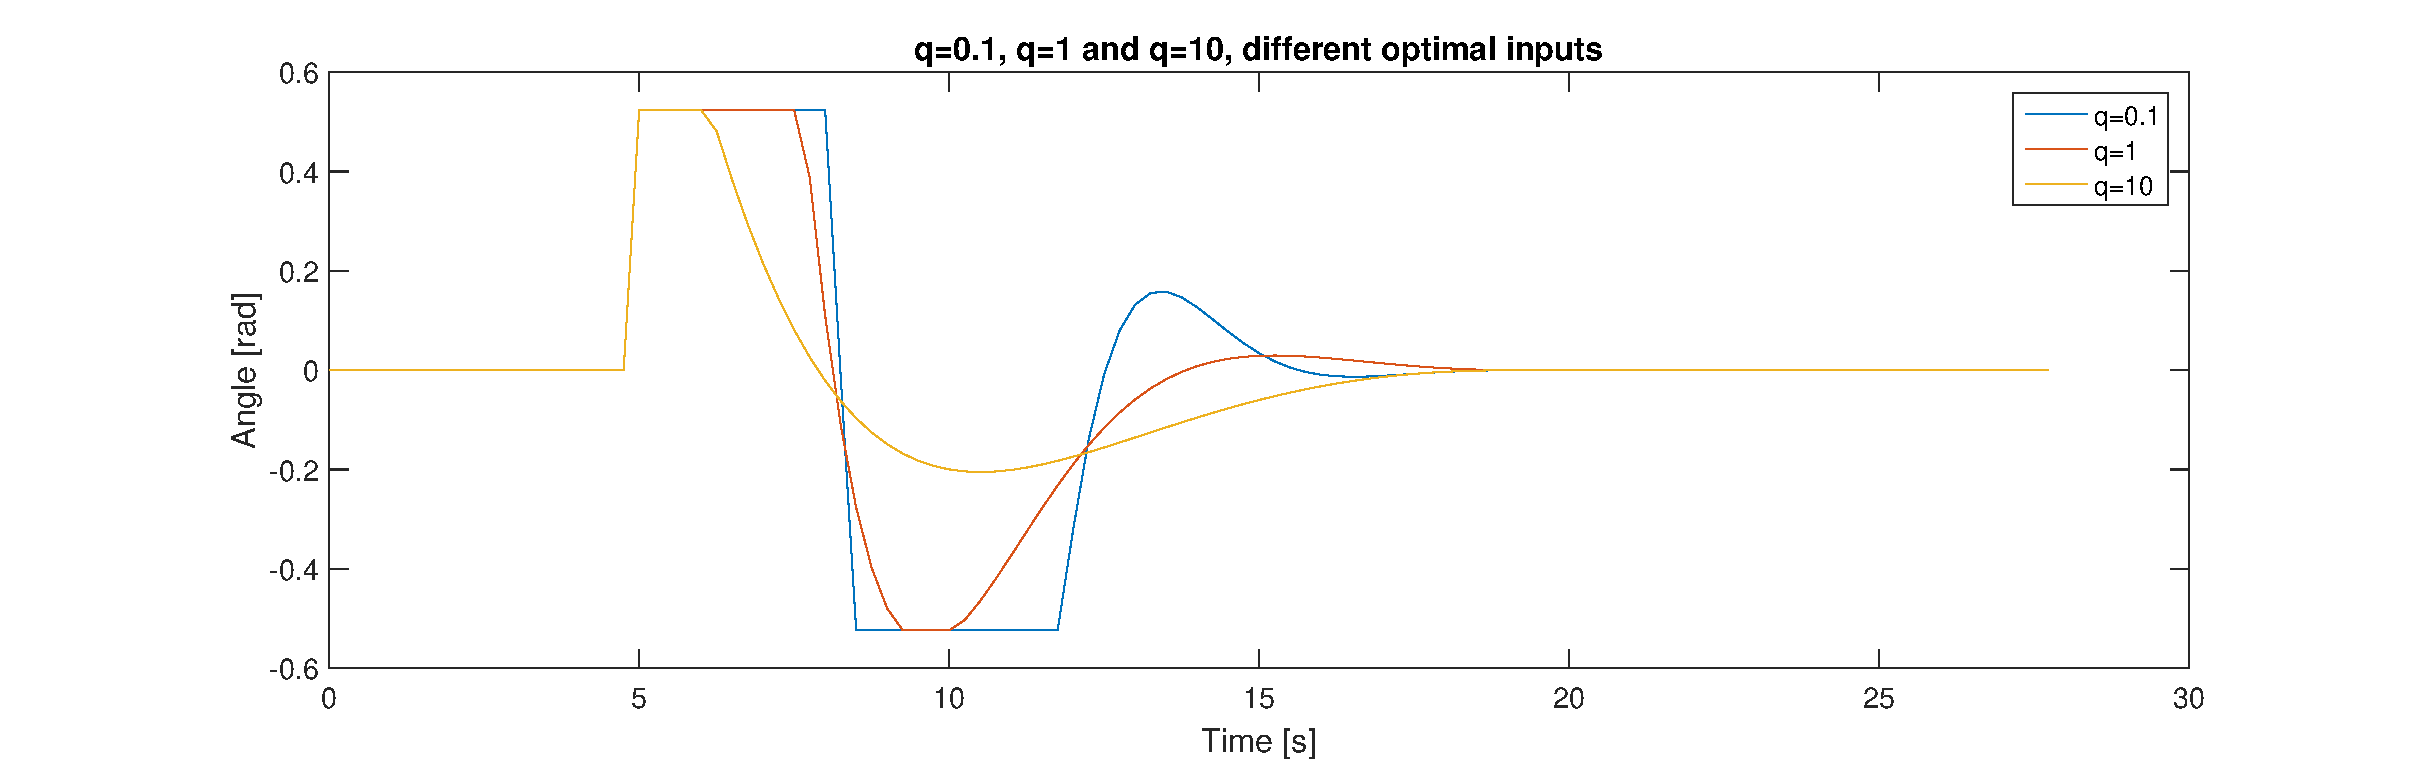
\includegraphics[width=1.2\textwidth]{task23_optimal_inputs.eps}}%
    \caption{Calculated optimal inputs}
    \label{fig:optimal_inputs}
\end{figure}

\begin{figure}[H]
    \centering
    \makebox[\textwidth][c]{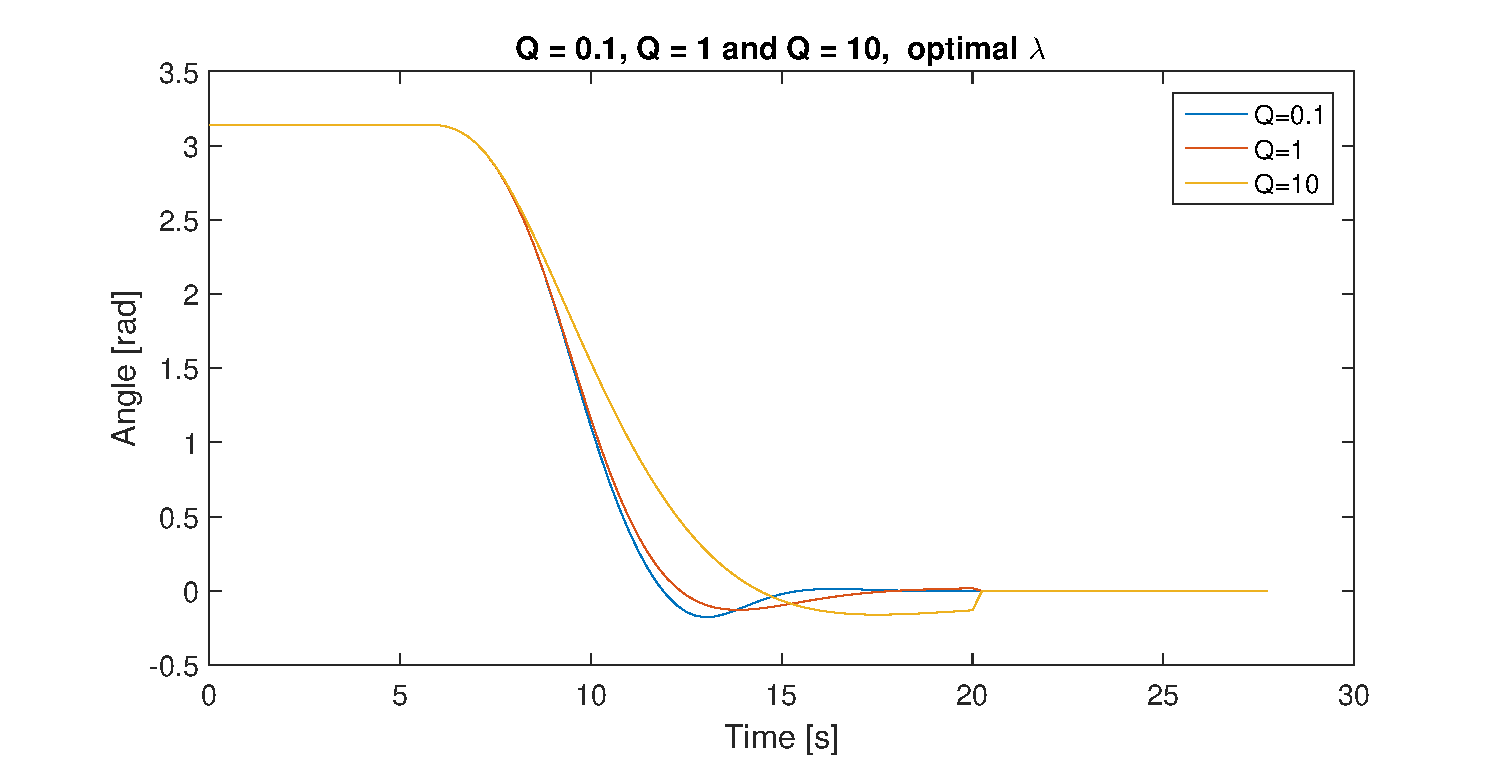
\includegraphics[width=1.2\textwidth]{optimal_lambda.eps}}
    \caption{Optimal $\lambda$ using LQ controller with different Qs.}
    \label{fig:optimal_lambda}
\end{figure}

The cost function to be minimized is $\phi = \sum_{i=1}^{N} (\lambda_i-\lambda_f)^2 + qp_{ci}^2$. The first term aims to penalize deviation from the reference point $\lambda_f$, while the second one penalizes inputs $p_{ci}$. The relative cost of the two terms is set using the weight q. This can be seen in \cref{fig:optimal_inputs}; optimal input trajectories with larger Q are associated with a higher cost on the input, and are therefore more damped compared to optimal inputs with smaller Q. This is also reflected in \cref{fig:optimal_lambda}; the optimal trajectory with the smallest weight is the fastest one, at the cost of some overshoot.

The smallest weight $Q=0.1$ gives the most aggressive control, but requires rapid changes in input, which might wear down the system over time. $Q=10$ on the other hand, seems rather slow. $Q=1$ seems like a good compromise; it is reasonably fast and not so hard on the actuators. In addition, \cref{fig:optimal_lambda} shows that it, at least in theory, gives the least amount of overshoot.

One downside of the cost function is that it does not include travel rate. So if the time horizon is not large enough, one might risk that it moves to the set point as fast as possible, without trying to stay there. In other words, it might have a high travel rate when it reaches the destination.

Another possible downside is the cost term $(\lambda_i - \lambda_f)^2$, which does not take into account that $\lambda_i = \lambda_ i + 2\pi$, resulting in very poor pathing if exposed to a large perturbation. On the other hand, it might be desirable to actually perform one or multiple revolutions.
\todo{finner vi flere ulemper?}
\clearpage

\subsection{Data and results}
The Simulink implementation can be found in Appendix \ref{appendix:B}. Zeros were added before and after the optimal input sequence. For the full Matlab code, see Appendix \ref{appendix:A}.

\begin{figure}[H]
    \centering
    \makebox[\textwidth][c]{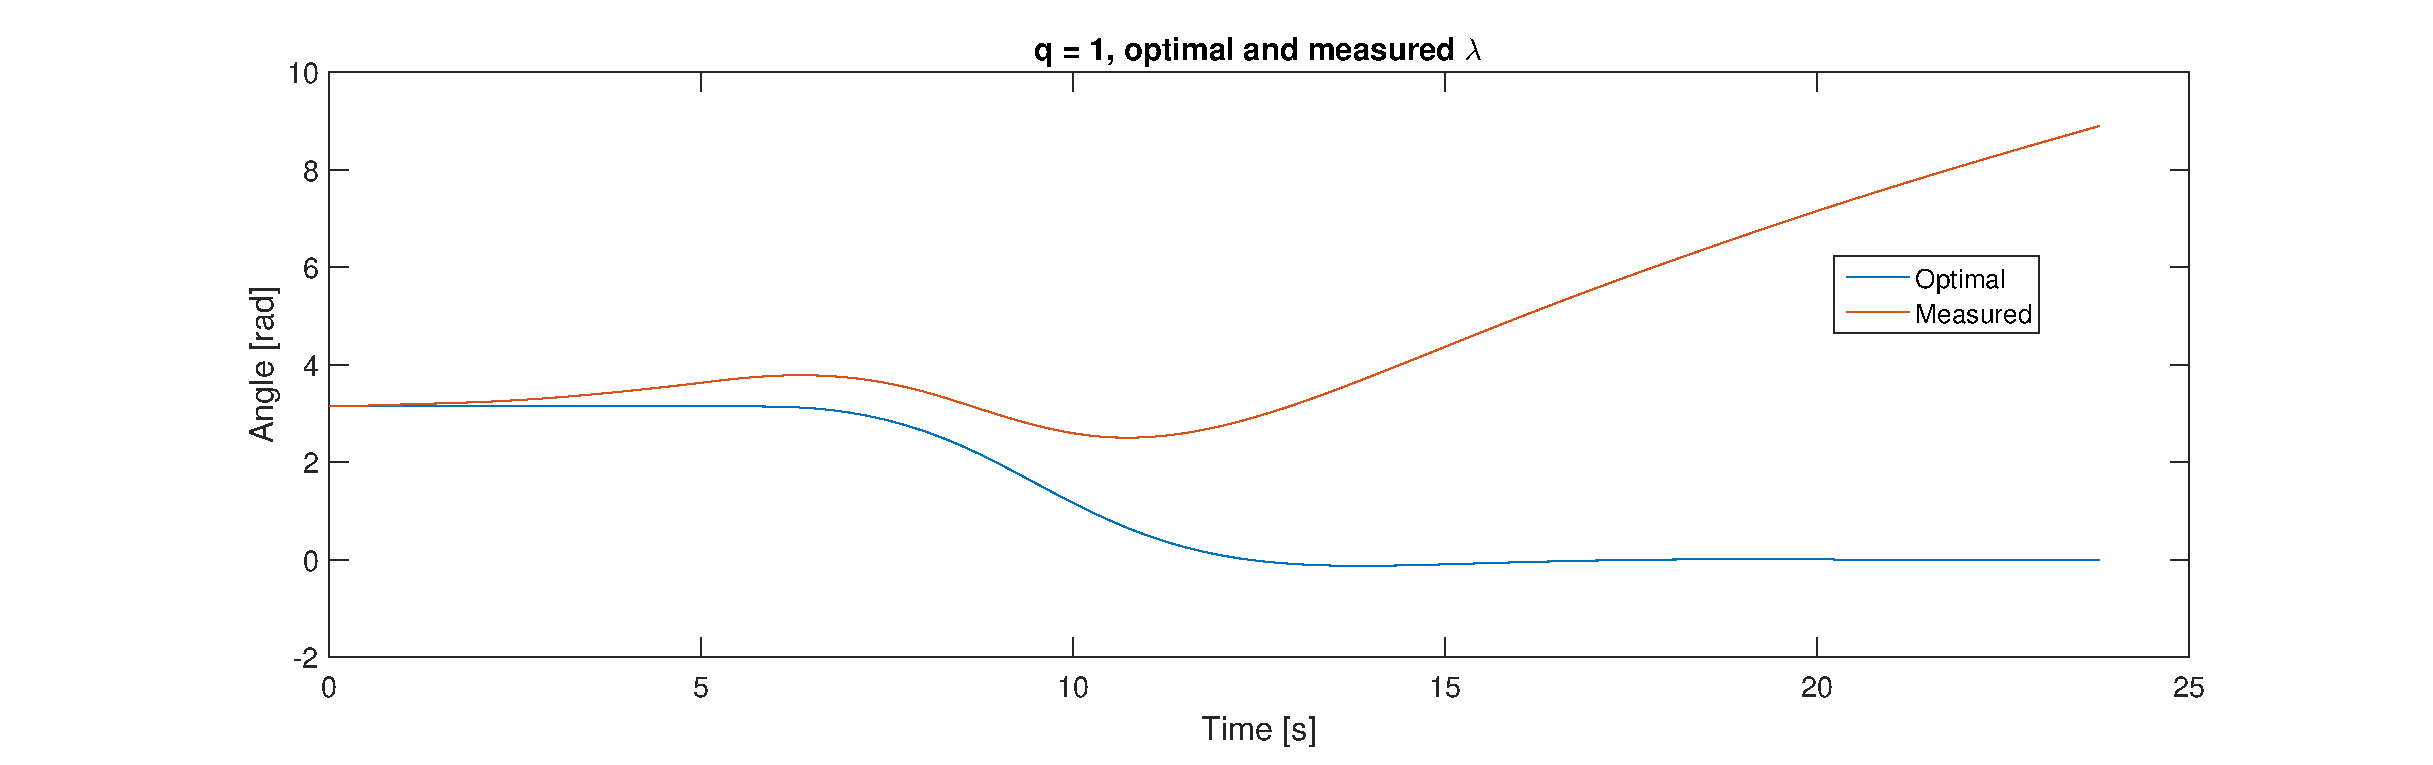
\includegraphics[width=1.2\textwidth]{optimal_and_measured_lambda.eps}}
    \caption{Optimal and measured $\lambda$ using LQ controller}
    \label{fig:my_label}
\end{figure}

The helicopter does not end in the desired point $x_f$. There seems to be a constant error in travel rate or pitch. This is largely \todo{er det flere grunner?} because of model inaccuracies; discretization errors from using forward Euler and linearization errors, in addition to inherent model errors/simplifications. Also, the system is affected by noise (e.g. wind currents) as well as measurement errors.

If our model was completely accurate, the helicopter would have followed the planned trajectory. However, since this never is the case, the fault lies in the regulator; there is no feedback for $\lambda$, so it has no way to correct for the model inaccuracies.

%\clearpage
